%  <-- ezzel lesznek jelölve a kommentek,
%a legtöbb dolgot jobb békénhagyni úgy ahogy van, általában csak {} közé vagy \section{} alá kell írni majd
%az ITKproc miatt nem kell megformáznod a szöveget tehát ezt mindenképpen hagyjátok a itt, valamint mindig legyen a dokumentum mappájában, hogy elérje a fordító
\documentclass[10pt, conference,a4paper]{ITKproc}

\usepackage[utf8]{inputenc}
\usepackage{graphicx}
\graphicspath{{images/}}
\usepackage{gensymb}
% correct bad hyphenation here

\hyphenation{pre-sence vi-su-alized si-mu-la-tions mo-le-cu-lar se-ve-ral cha-rac-te-ris-tic CoNSEnsX}


\begin{document}
% ide a {} közé írd a jegyzőkönyv címét
\title{RC tag mérési jegyzőkönyv}
% ezek gondolom egyértelműek, itt is mindig csak a {} szerkesszétek, valamint használhattok \\ sortöréshez, pl dátum hozzáírás stb
\author{\IEEEauthorblockN{Mátyás Antal}
\IEEEauthorblockA{(Supervisor: Attila Tihanyi)\\
Pázmány Péter Catholic University, Faculty of Information Technology and Bionics\\
50/a Pr\'ater street, 1083 Budapest, Hungary\\
\texttt{antal.matyas.gergely@hallgato.ppke.hu}}
}


\maketitle

\begin{abstract}
A mérés célja volt a RC tag megismerése és gyakorlati alkalmazása, valamint ennek áramkör módosító hatásának vizsgálata. A mérésre való felkészülés során átismételtük középiskolában az impedanciáról és látszólagos ellenállásról tanultakat, valamint a Fourier sorfejtés módszereit. \end{abstract}

\IEEEpeerreviewmaketitle
% innentől kezdve jönnek a feladatok
% \section{} Ezzel hozunk létre fejezetet, a {} közé pedig bármi írhatunk, általában úgyis "Feladat" és "összefoglalás"-t fogunk,
% a fejezetek alapjáraton számozódnak római számokkal tehát azt nem szükséges beleírni, 
% ha alfejezeteket akarunk létrehozni akkor \subsection{} subsubsection{} stb- vel tegyük
%példa:
\section{Mérendő objektumok}
A mérések során két ($R_1$ és $R_2$) ellenállást, valamint egy ($C_1$) kondenzátort használtunk. Első lépésként ezeknek értékét mértük meg az ELVIS Digital Multimeter segítségével. A következő értékeket kaptuk: \[R_1 = 0.974 k\Omega, R_2 = 0.11 M\Omega, C_1 = 0.096 \mu F\]

%%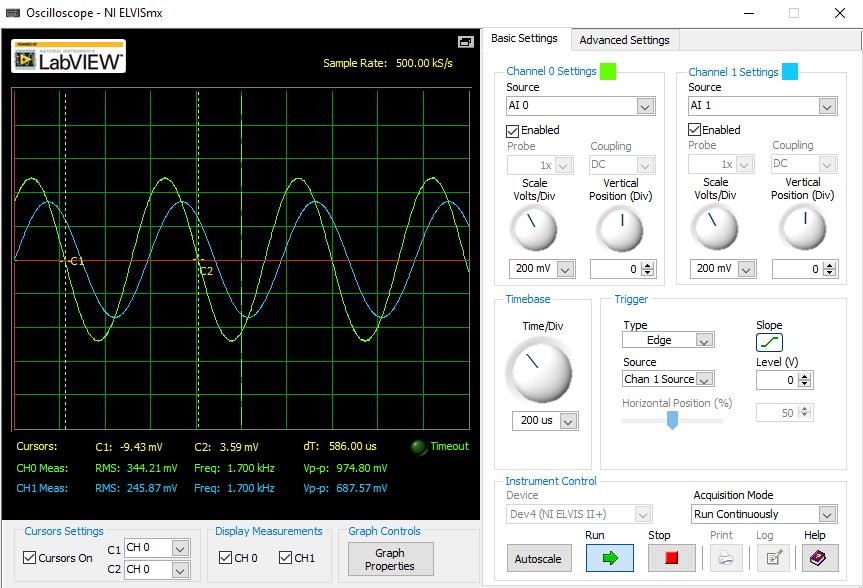
\includegraphics[scale=1]{1proba}

A mérések során minden esetben megmértük a mérőeszközben a nulla ellenállást, illetve feszültséget, és a Null Offset funkció használatával ezt automatikusan kivontuk a később mért értékekből, ezzel kiküszöbölve az offszet hibát. 

\section{Bemeneti impedancia mérése}
\subsection{Első összeállítás}

Első lépésben összeállítottuk a mérést a mérési utasításban feltüntetett módon, $Z_1 = R_1$ és $Z_2 = C_1$ értékekkel. A sorba kötött ellenállást és kapacitást a DUT+ és DUT- ELVIS kimeneti pontok közé kötve és az Impedance Analyzerrel vizsgálva a következő értékeket kaptuk:

\begin{table}[ht!]
\renewcommand{\arraystretch}{1.3}
\caption{Frekvencia - Amplitúdó}
\centering
\begin{tabular}{c||c}
\hline
\bfseries Frequency (Hz) & \bfseries Magnitude (kOhms) \\
\hline\hline
 10 & 162.04\\
\hline
 100 & 16.36\\
\hline
1000 & 1.92\\
\hline
10000 & 0.983\\
\hline
\end{tabular}
\end{table}
\begin{figure}[h]
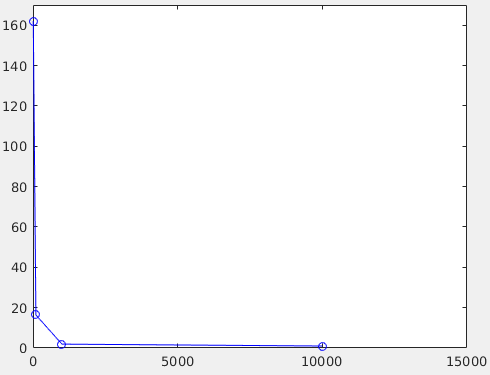
\includegraphics[scale=0.3]{1_f_m}
\centering

\end{figure}

\begin{table}[ht!]
\renewcommand{\arraystretch}{1.3}
\caption{Frekvencia - Fázisszög}
\centering
\begin{tabular}{c||c}
\hline
\bfseries Frequency (Hz) & \bfseries Phase (degrees) \\
\hline\hline
 10 & 270.95\\
\hline
 100 & 274.02\\
\hline
1000 & 300.94\\
\hline
10000 & 351.03\\
\hline

\end{tabular}
\end{table}

\begin{figure}[h]
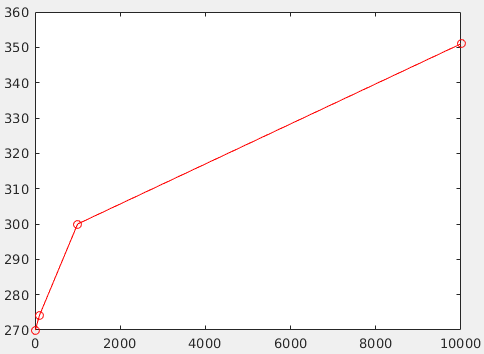
\includegraphics[scale=0.3]{1_f_p}
\centering

\end{figure}

\subsection{Második összeállítás}

A mérési utasítás 6. feladatát követve a mérési összeállítást a $Z_1 = C_1$ valamint $Z_2 = R_1$ értékekre módosítottuk, majd az előzővel azonos módon az ELVIS Impedance Analyzer segítségével különböző frekvenciákon vizsgáltuk. A mért értékek, valamint az ezek alkotta grafikonok alább láthatók: 

\begin{table}[ht!]
\renewcommand{\arraystretch}{1.3}
\caption{Frekvencia - Amplitúdó}
\centering
\begin{tabular}{c||c}
\hline
\bfseries Frequency (Hz) & \bfseries Magnitude (kOhms) \\
\hline\hline
 10 & 161.24\\
\hline
 100 & 16.35\\
\hline
1000 & 1.92\\
\hline
10000 & 0.983\\
\hline
\end{tabular}
\end{table}

\begin{figure}[h]
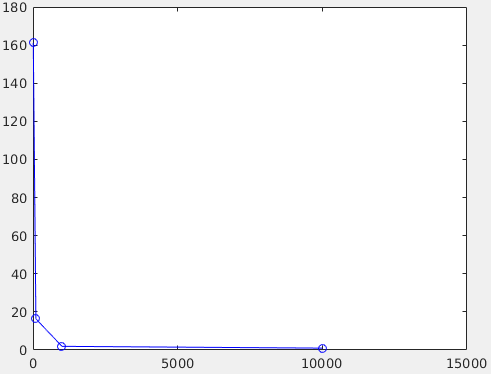
\includegraphics[scale=0.3]{2_f_m}
\centering

\end{figure}


\begin{table}[ht!]
\renewcommand{\arraystretch}{1.3}
\caption{Frekvencia - Fázisszög}
\centering
\begin{tabular}{c||c}
\hline
\bfseries Frequency (Hz) & \bfseries Phase (degrees) \\
\hline\hline
 10 & 273.68\\
\hline
 100 & 274.02\\
\hline
1000 & 300.96\\
\hline
10000 & 351.04\\
\hline

\end{tabular}
\end{table}
\begin{figure}[h]
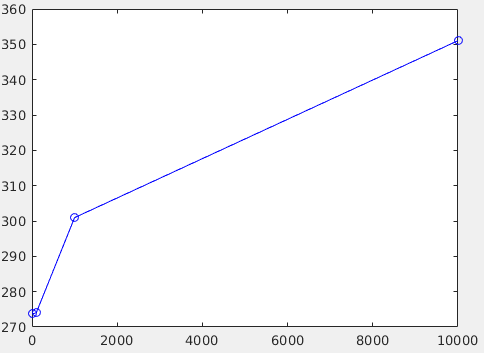
\includegraphics[scale=0.3]{2_f_p}
\centering

\end{figure}


\section{BODE Analyzer}
\subsection{Első összeállítás}

A mérési utasításban feltüntetett ábra alapján összeállítottuk a mérést $Z_1 = R_1$ valamint $Z_2 = C_1$ értékekkel, majd az ELVIS BODE Analyzere segítségével kirajzoltattuk a kapcsolás átviteli függvényét valamint fázisforgatását. Az utasítást követve az átviteli függvényt $10Hz - 10kHz$ tartományban vettük fel, dekádonként 5 méréponttal, valamint $0.2 V$ csúcsfeszültséggel. A BODE Analyzer grafikonját alább szemléltetjük: 
\begin{figure}[h]
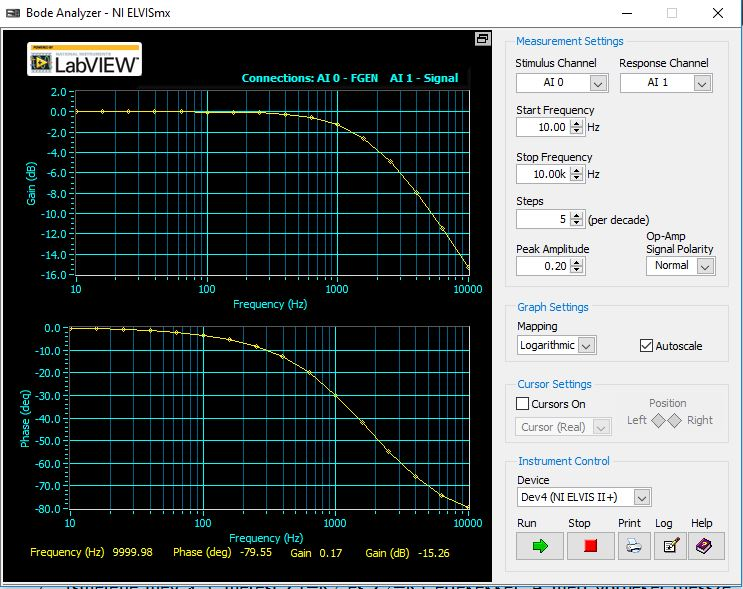
\includegraphics[scale=0.3]{bode_1}
\centering
\end{figure}


\subsection{Második összeállítás}
A második mérési összeállításban az Impedance Analyzerrel való vizsgálathoz hasonlóan módosítottuk a mért áramkört $Z_1 = C_1$ és $Z_2 = R_1$ értékekre. A BODE Analyzert használva ekkor a kirajzolt grafikon az alábbi:
\begin{figure}[h]
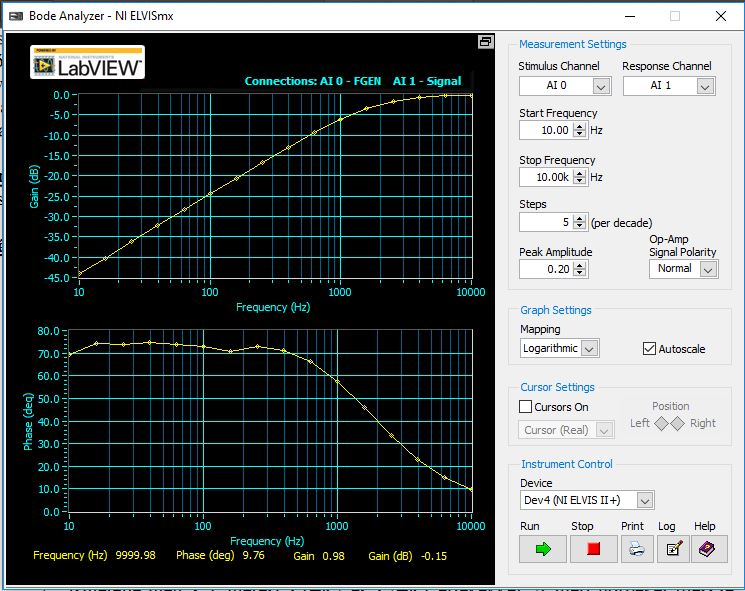
\includegraphics[scale=0.3]{bode_2}
\centering
\end{figure}

\subsection{Harmadik összeállítás}
A mérési összeállítást, ezután megvizsgáltuk $Z_1 = R_1$ valamint $Z_2 = R_2$ értékekkel is, ezt is ábrázoltuk a BODE Analyzer segítségével:
\begin{figure}[h]
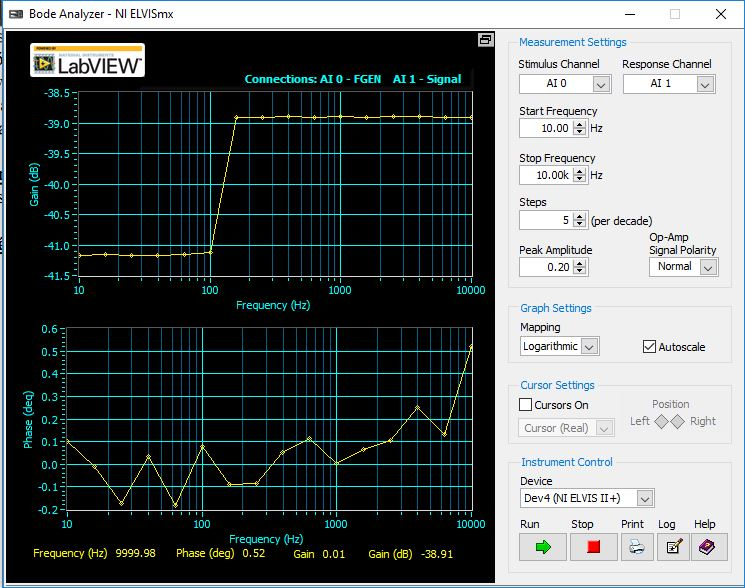
\includegraphics[scale=0.3]{bode_3}
\centering
\end{figure}

\section{Magyarázat}
Az első összeállításnál az ábráról leolvasható, hogy a frekvencia növekedésével csökken a reaktancia, 	ezért a feszültség amplitúdója is csökken, tehát egy aluláteresztő szűrőrről van szó, mely az alacsony frekvenciájú jeleket átengedi, a magas frekvenciájúakat azonban csillapítja. 
\\
\\
A második öszeállítás az ábra alapján éppen ellenkezője az elsőnek, hiszen minél nagyobb a frekvencia, annál kevésbé csökken a frekvencia amplitúdója, vagyis az összeállítás egy felüláteresztő szűrőt képez. 
\\
\\
A harmadik összeállításban, mivel az áramkör csak ellenállásokból áll, reaktanciát nem mérhetünk, így konstans 0 értékre számíthatunk. Az ábra ettől itt nagyon kis mértékben tér el, a felső grafikonon való ugrás a műszer méréshatárváltásának tudható be. 

\section{Oscilloscope}
\subsection{Szinuszos gerjesztés}
A feladat során az ELVIS Oscilloscope segítségével mértük a fázisszöget az AI0 és AI1 csatornák között, szinuszos gerjesztés esetén. 
A kirajzolt ábra az alábbi:
\begin{figure}[h]
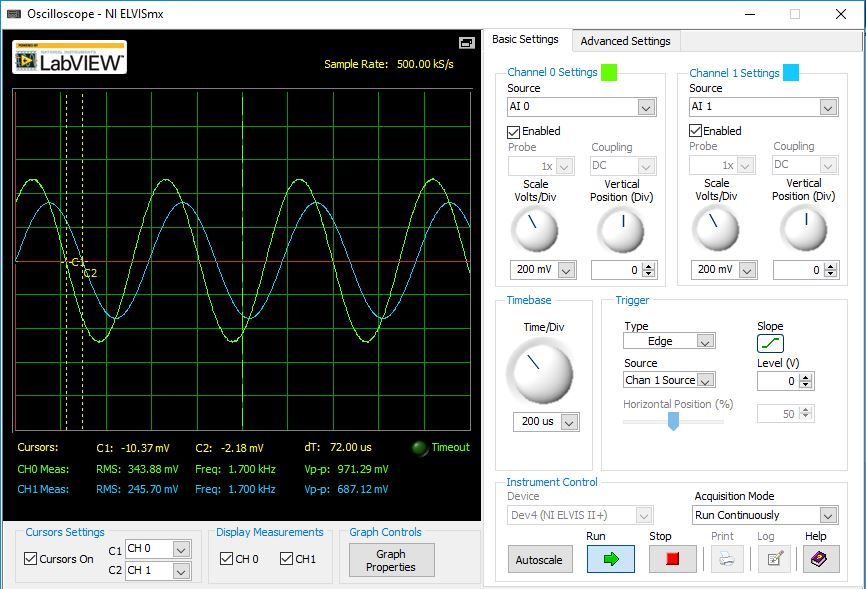
\includegraphics[scale=0.3]{oscil_1}
\centering
\end{figure}
A csatornák közötti fáziseltérést a pediódusuk közötti idők összehasonlításával tudtuk meghatározni. Egy teljes periódus idejét arányosítottuk 360\degree -kal. Az ábráról leolvasott periósusidő $528\mu s$, így $1\mu s = \frac{360}{528} \degree$, a leolvasott időeltérés a két jel periódusa között pedig $72\mu s$, tehát a fáziseltérés $72*\frac{360}{586} = 16.587 \degree$. 

\subsection{Mérési összeállítás}
A következő feladat volt kiszámítani azt a frekvenciát, ahol a kapacitás látszólagos ellenállásának abszolút értéke megegyezik az ellenállás értékével, majd ekkora frekvenciájú, $1V$ csúcsértékű négyszögjelet kapcsolni az árakör bemenetére, majd oscilloscope segítégével kirajzolni a bemenő és kimenő jelalakot, és kiszámítani az azok közötti fázisszöget. \[R = \frac{1}{2*\pi * f*C} \to f = \frac{1}{2*\pi *R*C}\]
Az így kapott frekvencia: $1.7 kHz$.
Az ELVIS signal generatoron ezt az értéket beállítva az oscilloscope az alábbi ábrát rajzolja ki:
\begin{figure}[h]
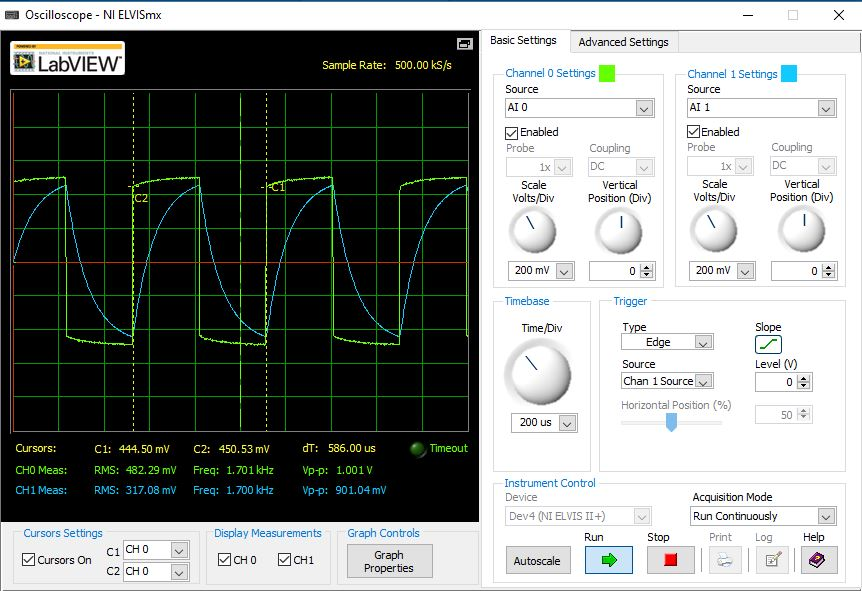
\includegraphics[scale=0.3]{oscil_2}
\centering
\end{figure}
A jelalak nyilvánvalóan különböző, azonban a jelek amplitúdója egyértelműen megegyezik. 

\section{Dynamic Signal Analyzer}
A következő feladatban az előre megadott paraméterek alapján beállított (Voltage Range: +/- 10V, Frequency Span: 10000Hz, Resolution: 400 lines, Hamming) függvénygenerátorral mértünk. A kapott diagrammot vizsgálva a felharmonikusok frekvenciája: 105Hz, 320Hz, 535Hz, 755Hz, melyből látszik, hogy a felharmonikusok az alapharmonikus frekvenciájának kétszeresével követik egymást. 
\subsection{Fourier sor}
Tetszőleges függvény Fourier-sora: $f(x) = \frac{a_0}{2} + \sum_{k=1}^{\infty} (a_k*cos(kx)+b_k*sin(kx))$, ahol jelen esetben $f(x)$ a négyszögjel függvénye lesz. 
A kapott értékeket a négyszögfüggvény matematikai Fourier-analízisével összevetve egy $sin(x)/x$-hez hasonló gráfot kaptunk(abszolútértékben). 
\[\frac{4}{\pi} * \sum(\frac{1}{2k-1}*sin((2k-1)\omega *t))\]
A függvény maximumai ott vannak, ahol $sin((2k-1)\omega *t) = 1$, ezek az ábrán látható csúcsok, melyek értéke a $b_k$ együtthatók miatt csökken. 
\section{Jellemzés/Magyarázat}
A mérések alapján megállapítható, hogy az első mérési összeállításban, azaz $Z_1 = R_1$ és $Z_2 = C_1$ esetén aluláteresztő, csillapításos feszültségosztót kapunk, míg a második összeállításban, azaz $Z_1 = C_1$ és $Z_2 = R_1$ esetén erősítéses felüláteresztőt. 
%Ha szeretnéd hogy az adott fejezet ne legyen számozva használj \section*{} -t, pl Acknowledgements


% Az egyenletekre, táblázatokra, listákra stb. itt nem térnék ki, ahhoz mindenképp érdemes kicsit utána olvasni

% A references mindig a legutolsó fejezet lesz

%  minden hivatkozás elnevezünk, ezzel a névvel fogunk hivatkozni a szövegen belül
% \bibitem{} <- hivatkozásnév
% A hivatkozás formája legjobban a példa dokumentumban látszik a tanárúr honlapján, általában: szerző, olvasott anyag neve, közreműködők, hely, év
% a szövegben pedig \cite{Megadott hivatkozásnév} -vel hivatkozunk


% példa:


% Ez a rész mindig marad:---------
\bibliographystyle{ieeetr}
%\bibliography{references}


% that's all folks
\end{document}